% Made up for the tikra benchmark.
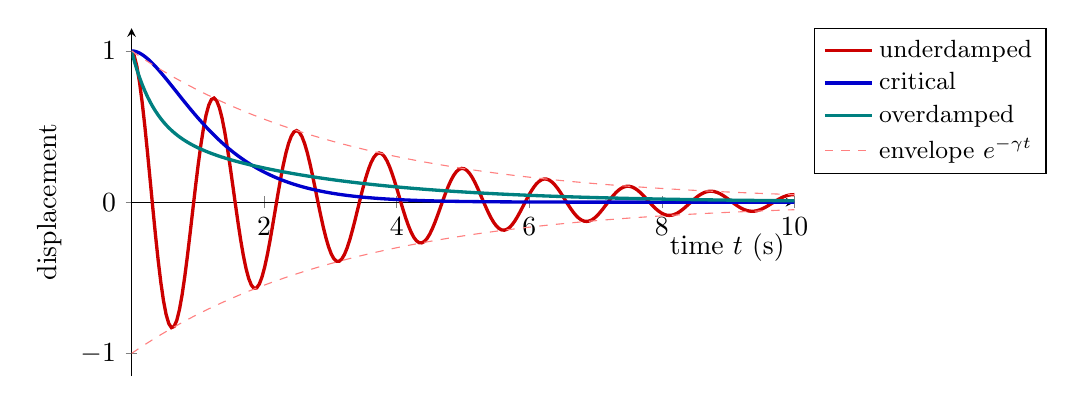
\begin{tikzpicture}
\begin{axis}[width=10cm, height=6cm, xmin=0, xmax=10, ymin=-1.15, ymax=1.15, domain=0:10,
    samples=250, xlabel={time $t$ (s)}, ylabel={displacement}, axis x line=middle,
    axis y line=left, xlabel style={anchor=north east, at={(axis description cs:1,0.5)}, yshift=-8pt},
    legend pos=outer north east, legend cell align=left, legend style={font=\small}]
  \addplot[red!80!black, very thick] {exp(-0.3*x)*cos(deg(2*pi*0.8*x))};
  \addlegendentry{underdamped}
  \addplot[blue!80!black, very thick] {(1 + 1.5*x)*exp(-1.5*x)};
  \addlegendentry{critical}
  \addplot[teal, very thick] {0.5*(exp(-0.4*x) + exp(-3*x))};
  \addlegendentry{overdamped}
  \addplot[red!50, dashed] {exp(-0.3*x)};
  \addlegendentry{envelope $e^{-\gamma t}$}
  \addplot[red!50, dashed, forget plot] {-exp(-0.3*x)};
\end{axis}
\end{tikzpicture}
